% Destination labels use only the top-level transaction address and bundled constants.
\documentclass[border=6pt]{standalone}
\usepackage{tikz}
\usetikzlibrary{arrows.meta}
\begin{document}
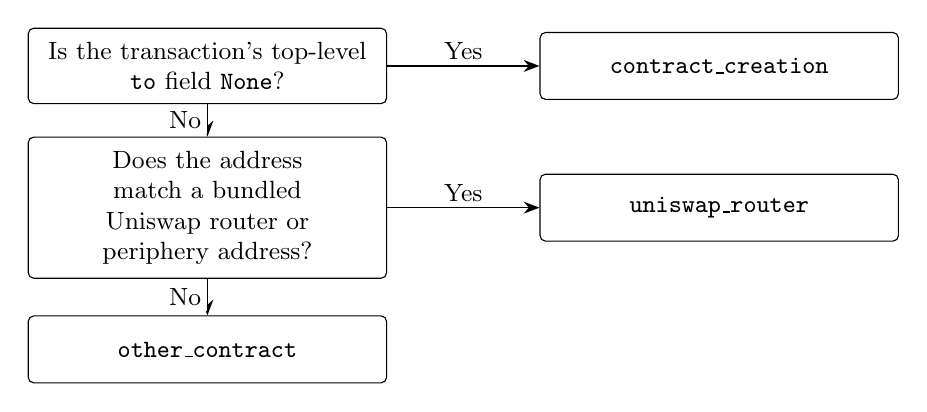
\begin{tikzpicture}[
  box/.style={draw, rounded corners=2pt, align=center, text width=4.2cm,
    minimum height=0.85cm, inner sep=5pt, font=\small},
  arrow/.style={-Stealth, semithick},
  label/.style={font=\small, fill=white, inner sep=2pt}
]
\node[box] (missing) at (0,0) {Is the transaction's top-level\\\texttt{to} field \texttt{None}?};
\node[box] (creation) at (6.5,0) {\texttt{contract\_creation}};
\node[box] (listed) at (0,-1.8) {Does the address match a bundled\\Uniswap router or periphery address?};
\node[box] (router) at (6.5,-1.8) {\texttt{uniswap\_router}};
\node[box] (other) at (0,-3.6) {\texttt{other\_contract}};
\draw[arrow] (missing) -- node[label,above] {Yes} (creation);
\draw[arrow] (missing) -- node[label,left] {No} (listed);
\draw[arrow] (listed) -- node[label,above] {Yes} (router);
\draw[arrow] (listed) -- node[label,left] {No} (other);
\end{tikzpicture}
\end{document}
